\begin{figure}[H]
    \centering
    \begin{subfigure}{0.3\textwidth}
        \centering
        \includegraphics[width=0.9\textwidth]{escala/city_13_viz.png}
        \caption{~\texttt{vizinho}.}
    \end{subfigure}%
    \hspace{8pt}
    \begin{subfigure}{0.3\textwidth}
        \centering
        \includegraphics[width=0.9\textwidth]{escala/city_13_bil.png}
        \caption{~\texttt{bilinear}.}
    \end{subfigure}
    \\[8pt]
    \begin{subfigure}{0.3\textwidth}
        \centering
        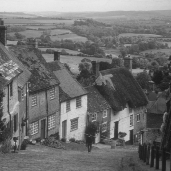
\includegraphics[width=0.9\textwidth]{escala/city_13_bic.png}
        \caption{~\texttt{bicubica}.}
    \end{subfigure}%
    \hspace{8pt}%
    \begin{subfigure}{0.3\textwidth}
        \centering
        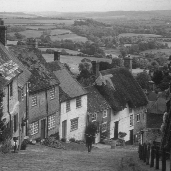
\includegraphics[width=0.9\textwidth]{escala/city_13_lag.png}
        \caption{~\texttt{lagrange}.}
    \end{subfigure}

    \caption{Escalonamento com $S_x = S_y = 1/3$ aplicado em \texttt{city.png} ($512 \times 512$).}
    \label{fig:esc:13}
\end{figure}